\chapter{Methodology}
This chapter begins with an overview of different segmentation types, highlighting their characteristics and differences. Then, various \acrfull{vit} architectures are introduced and discussed in detail. The model selected for this thesis is then presented, along with a comprehensive explanation of the modifications made to the attention mechanism, particularly the implementation of central self-attention and the reasoning behind its adoption. Afterward, the evaluation metrics employed to assess model performance are described. The chapter concludes with implementation details, describing the model's construction and deployment using Python.


\section{Image Segmentation}
Image segmentation is a subfield of computer vision that focuses on interpreting visual content by grouping regions in images or videos based on their underlying classes, with labels providing the semantic meaning of those classes. Depending on the required level of detail, segmentation is typically categorized into three main types: semantic segmentation, instance segmentation, and panoptic segmentation. It plays an important role in applications such as autonomous driving, medical image analysis, video surveillance, and image editing \cite{zhou2024imagesegmentationfoundationmodel}. The following section presents the key differences between semantic, instance, and panoptic segmentation.


\subsection{Semantic Segmentation}
The task of semantic segmentation consists of assigning a category label to every pixel in an image. This process allows for a high-level understanding of visual scenes by identifying and localizing various object classes and regions within the image \cite{zhou2018semanticunderstandingscenesade20k}. The goal is to produce a dense, per-pixel classification map in which pixels belonging to the same category (e.g., sky, road, person) are grouped together, regardless of object instances. Semantic segmentation is critical for interpreting scene layout and contributes significantly to applications that require detailed comprehension of visual data.


\subsection{Instance Segmentation}
The process of identifying and distinguishing each unique object instance in an image is known as instance segmentation  \cite{ke2021masktransfinerhighqualityinstance}. Unlike semantic segmentation, which assigns a category label to every pixel without distinguishing between different objects of the same class, instance segmentation treats each object's appearance as a separate entity. This means it not only classifies each pixel but also associates it with a specific instance of an object. Instance segmentation combines object detection and pixel-wise segmentation to generate high-quality masks that accurately capture the shapes and boundaries of individual objects, even when they overlap. The latter is called mask prediction. Compared to semantic segmentation it is significantly more complex due to the need to handle varying numbers of objects per image and to differentiate between closely located or overlapping instances of the same class.

\medskip

First, object detectors identify candidate object regions, typically using a region proposal network, and then a segmentation branch generates binary masks that accurately describe the shape of each object instance within its bounding box. The Mask Transformer method makes earlier techniques better by refining coarse mask predictions at the object boundaries using a Transformer-based architecture, enhancing accuracy particularly at fine-grained edges.


\subsection{Panoptic Segmentation}
Panoptic segmentation is a unified computer vision task that combines the goals of semantic and instance segmentation \cite{kirillov2019panopticfeaturepyramidnetworks}. Specifically, it is about assigning a semantic label to each pixel in an image (e.g. road, sky, person, animal) and at the same time distinguishing between individual object instances for \enquote{thing} classes (e.g.~separating multiple persons or animals) and treating \enquote{stuff} classes (e.g.~sky or grass) as amorphous regions without distinct instances.

\medskip

Panoptic segmentation works by simultaneously generating two outputs: one for instance segmentation and one for semantic segmentation. In the Panoptic \gls{fpn} model mentioned in the paper \cite{kirillov2019panopticfeaturepyramidnetworks}, a shared \gls{fpn} backbone is used to extract multi-scale features. On top of this backbone, a region-based branch (as in Mask R-CNN) is used for instance segmentation, while a lightweight dense-prediction branch is added for semantic segmentation. These two outputs are then merged through a post-processing step to ensure each pixel is assigned exactly one label and, if applicable, an instance \acrshort{id}.

\medskip

The key difference from instance segmentation is that panoptic segmentation also includes semantic segmentation of stuff classes, thereby providing a complete pixel-level understanding of the entire scene and not just individual objects. In contrast, instance segmentation focuses only on distinguishing individual object instances, typically omitting the background or amorphous regions. Panoptic segmentation addresses both objectives.


\subsection{Choice of Segmentation Method}
Given the availability of annotated \gls{3d} training data of shoe scans (see also chapter \ref{data_preparation}), semantic segmentation is employed in this thesis to enable accurate classification of components within a given volume. 



\section{Survey of Evaluated Vision Transformer Models}
Since this work focuses on the implementation and evaluation of a model for \gls{3d} semantic segmentation of high-resolution \gls{ct} scans of packed shoes, the next section discusses \gls{vit} methods that are suitable for this segmentation task.

\medskip

Selecting an appropriate model architecture is an important step in the design of an efficient deep learning pipeline, particularly when working with limited but memory-intensive volumetric data. Unlike regular vision tasks with dense and uniformly sized \gls{2d} images, the high-resolution voxel-based inputs in this project impose unique computational and architectural constraints. These include a cubic input space, sparse meaningful content, and extremely high memory requirements, which render many established \gls{2d} or video-based Transformer models unsuitable in their default configurations. Furthermore, the anisotropy and sparsity of the \gls{3d} input data call for architectures that can operate efficiently without compromising spatial resolution or contextual awareness. As a result, models must be carefully assessed not only for their raw performance but also for their ability to generalize within the constraints of volumetric imaging.

\medskip

To determine if the architecture is suitable, a detailed analysis of different types of Transformer variants, such as \gls{avit} \cite{du2024avitadaptingvisiontransformers}, \gls{efficientvit} \cite{liu2023efficientvitmemoryefficientvision}, \gls{shvit} \cite{yun2024shvit}, and \gls{tevit} \cite{yang2022temporallyefficientvisiontransformer} is conducted. \gls{shvit} was finally selected and analyzed in detail, focusing on their structural design, attention mechanisms, and scalability with respect to large \gls{3d} inputs. 

\medskip

An important criterion for inclusion or exclusion in the model selection process is not only the runtime performance but also memory efficiency. Equally relevant are the simplicity and architectural transparency of the model, which directly impact the ease of adaptability and extensibility. For example, being able to add extra parts for semantic segmentation easily and without interfering with the main components is crucial for adjusting a model to specific tasks. Therefore, models that demonstrate memory scaling and allow for clean architectural structure are prioritized in the subsequent evaluation.




\subsection{Semantic Segmentation Transformer (SegFormer)} \label{sec:segformer}
SegFormer is another Vision Transformer (\gls{vit}) architecture that employs a series of efficient self-attention blocks within its encoder \cite{xie2021segformersimpleefficientdesign, perera2024segformer3defficienttransformer3d}. The encoder is organized into four hierarchical stages, each designed to progressively reduce spatial resolution while enriching feature representations. The process starts with an overlapping patch embedding mechanism, in which small, overlapping regions are extracted from the input image and linearly projected into feature vectors. In the first stage, the patch kernel size is set to 7 with a stride of 4 and padding of 3; in subsequent stages, the patch kernel size is reduced to 3 with a stride of 2 and padding of 1. This design halves the spatial resolution at each stage while simultaneously increasing the number of feature channels.

\medskip

Within each stage, the feature map passes through multiple transformer blocks. Each block starts with an efficient self-attention mechanism that reduces the sequence length for keys and values by a fixed factor to drastically cut computational cost. This is immediately followed by a Mix-\gls{ffn}: a feed-forward network that combines a linear \gls{mlp} with a lightweight, data-driven convolution, preserving spatial information without relying on fixed positional embeddings. At the end of each stage, patches are merged again via \enquote{Overlap Patch Merging} to produce the next deeper feature level. The result is a multi-level feature hierarchy that seamlessly integrates local detail with global context (see also figure \ref{Architecture_of_Segformer}).

\medskip

SegFormer's decoder follows an intentionally lightweight design, avoiding the use of complex convolutional operations. To begin, each of the four multi-scale feature maps generated by the encoder is linearly projected to ensure a consistent number of channels across all stages. These feature maps are then resized via bilinear interpolation to the same spatial resolution, typically one-fourth of the original input size.

\medskip

After alignment, the features are concatenated and passed through a simple \gls{mlp}, which fuses them into a unified representation. A final linear layer then produces the pixel-wise segmentation map, assigning class probabilities to each location.

\begin{figure}[H]
	\centering
	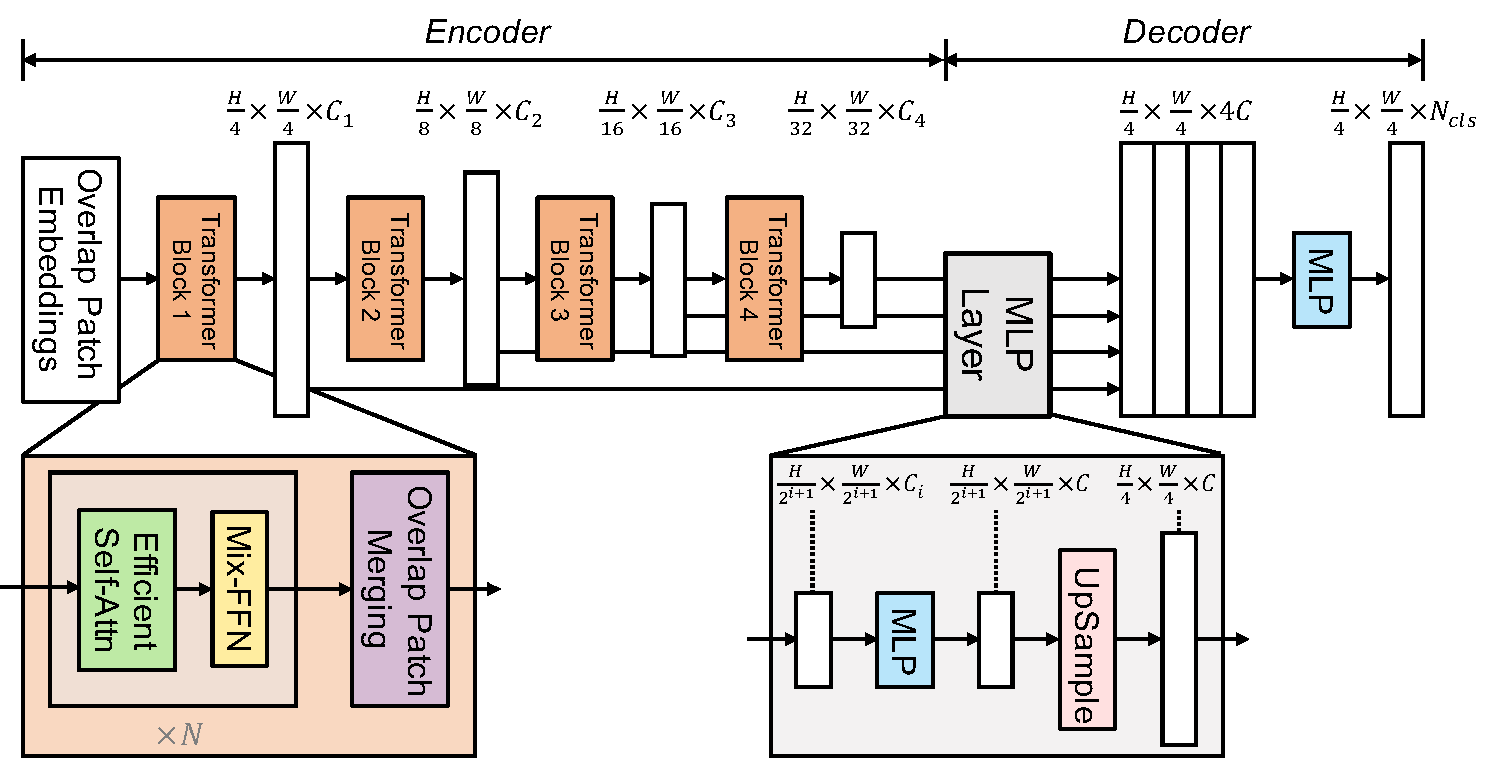
\includegraphics[width=1.0\textwidth]{./images/Segformer_architecture.pdf}
	\caption[Architecture of SegFormer]{Architecture of SegFormer. Image taken from \cite{xie2021segformersimpleefficientdesign}.}
	\label{Architecture_of_Segformer}
\end{figure}


%%%%%%%%%%%%%%%%%%%%%%%%%%%%%%%%%%%%%%%%%%%%%%%%%%%%%%%%%%%%%%%%

\subsection{Adapting Vision Transformer (AViT)}
\gls{avit} is a vision-transformer-based model specifically designed for skin lesion segmentation on small dermoscopic datasets. The idea behind \gls{avit} is that a large pre-trained Vision Transformer backbone already encodes the essential visual representations, e.g.~spatial details, boundaries, and texture \cite{du2024avitadaptingvisiontransformers}. Only a small subset of the model's parameters needs to be adapted to address new, specialized tasks. Instead of fine-tuning the entire \gls{vit} model for each new task, \gls{avit} keeps the backbone's weights completely frozen to preserve the learned representations and reduce memory usage, as these parameters do not need to be duplicated across different datasets. This is achieved by inserting two lightweight modules: a prompt generator and an adapter (see figure \ref{Architecture_of_AVIT}).

\begin{figure}[H]
	\centering
	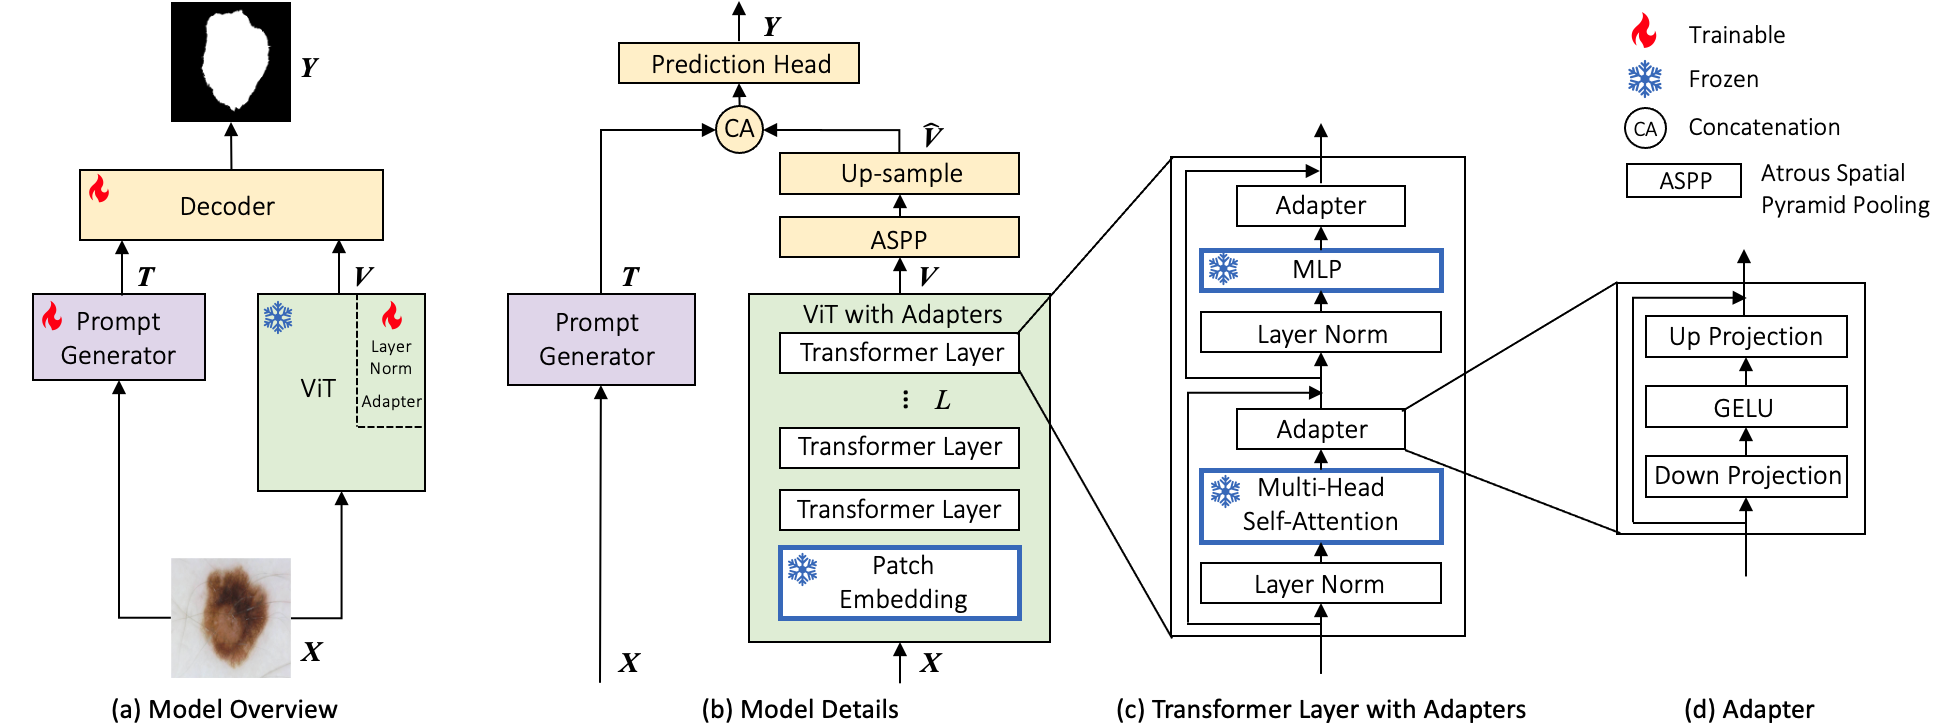
\includegraphics[width=1.0\textwidth]{./images/AViT_architecture.png}
	\caption[Architecture of AViT]{Architecture of AViT: (a) Model overview with prompt generator and a large pre-trained ViT backbone with adapters, and a compact decoder. (b to d) Model details. During training, all modules in (b,c,d) contoured with blue borders are frozen. Image and text taken from \cite{du2024avitadaptingvisiontransformers}.}
	\label{Architecture_of_AVIT}
\end{figure}

The prompt generator extracts information from images by leveraging the inductive biases of \glspl{cnn}, which provide the ability to capture spatial details, boundaries, and textures even with limited training data. It generates a set of prompt embeddings that consists of seven convolutional layers. Before being fed into the \gls{vit}'s \gls{mhsa}, these prompt embeddings are appended to the beginning of the patch embeddings sequence. They influence the representation learned at each layer and remain throughout the transformer's stages. During training, only the parameters of the prompt generator and the adapter modules are updated, while the weights of the pre-trained backbone remain frozen. This design enables domain- and context-specific conditioning without increasing memory consumption or duplicating the frozen backbone for each new dataset.

\medskip

Adapters are integrated into skip connections of each transformer block, following a bottleneck architecture composed of a down-projection to reduce hidden dimensionality and an up-projection to restore it. Positioned between the \gls{mhsa} layers and the \gls{ffn}, the adapters are the only components updated during training, while the parameterized pre-trained backbone remains frozen. This configuration reduces memory consumption by over 60\%\footnote{The fully fine-tuned base model with 367.2\,M parameters (91.8\,M$\times$4), \gls{avit} requires only 140.2\,M parameters, consisting of a single shared \gls{vit} backbone (85.8\,M) and 13.6\,M per dataset for adapters and the prompt generator, resulting in a memory reduction of approximately 60\%.} by avoiding redundancies of the backbone across datasets. Moreover, the compact parameterization of the adapters minimizes redundancy without significantly limiting the model's representational capacity, enabling efficient adaptation under constrained data conditions.

\medskip

During training, \gls{avit} benefits not only from a significantly reduced number of trainable parameters, but also from a substantially lower peak \gls{gpu} memory footprint. Classical \gls{mhsa} scales quadratically with the input sequence length, which becomes computationally prohibitive for high-resolution volumetric inputs such as $256^{3}$ voxels (resulting in approximately $4{,}096$ patches at a patch size of $16^{3}$). \gls{avit} addresses this challenge by freezing the large Vision Transformer backbone and introducing only a small number of additional prompt tokens. In practice, a patch size of $16^3$ voxels reduces the sequence length to around $4{,}096$ tokens, making the use of transformer-based models on volumetric data feasible without exceeding memory constraints\footnote{The number $4{,}096$ results from dividing the volume size $256^3$ by the patch volume $16^3$ (i.e., $256^3 / 16^3 = 4,096$ patches). The number $4{,}096$ is an example of a smaller volume such as $256^3$ voxels: $256^3 / 16^3 = 16^3 = 4{,}096$. Adjust numbers based on actual use cases.}. 



\subsection{Efficient Vision Transformer (EfficientViT)}
\gls{efficientvit} was designed based on a so-called sandwich layout to achieve high inference speed \cite{liu2023efficientvitmemoryefficientvision}. The bottleneck arises from memory-intensive and computationally inefficient operations such as tensor reshaping or elementwise functions in the \gls{mhsa} block. Instead of the alternating arrangement of self-attention and feedforward layers, this bottleneck can be reduced by adopting a sandwich layout in the \gls{efficientvit} block. In this design, a cascaded group attention block is placed between two blocks, each consisting of a token interaction layer and an \gls{ffn} layer. 

\medskip

Acceleration in the cascaded group attention block is achieved by assigning each attention head a different split of the input. This reduces the computational load by a factor equal to the number of heads while simultaneously increasing the diversity of the attention maps without introducing any additional parameters. 
\begin{figure}[H]
	\centering
	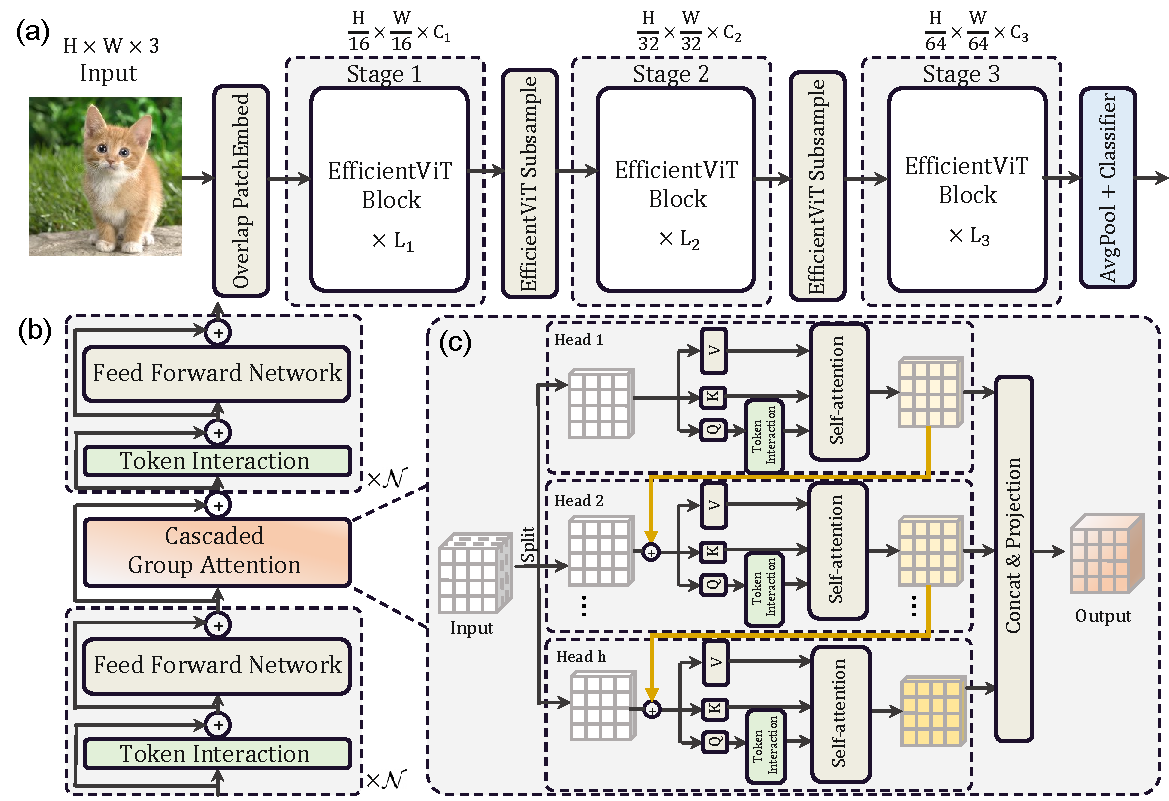
\includegraphics[width=1.0\textwidth]{./images/EfficientViT_architecture.pdf}
	\caption[Architecture of EfficientViT]{Architecture of EfficientViT: (a) Overview; (b) Sandwich Layout block; (c) Cascaded Group Attention. Image and text taken from \cite{liu2023efficientvitmemoryefficientvision}.}
	\label{Architecture_of_EfficientViT}
\end{figure}



\subsection{Temporally Efficient Vision Transformer (TeViT)}
\gls{tevit} was developed for \gls{vis}, combining a hierarchical transformer backbone with multiple query‑based heads for instance segmentation and temporal association (tracking) \cite{yang2022temporallyefficientvisiontransformer}. The backbone is built on a \gls{pvt} variant that reduces the number of patch tokens to lower memory requirements. The Messenger Shift mechanism injects temporal context by shifting lightweight messenger tokens between successive frames, without any trainable parameters, thereby enabling efficient temporal fusion with minimal memory and compute overhead.

\medskip

Given a sequence of video frames, Patch Merging successively generates multi‑scale pyramid feature maps (with strides of 4, 8, 16, and 32), reducing spatial resolution at each stage. At the same time, messenger tokens are appended to each frame and then shifted across adjacent frames via the Messenger Shift mechanism, facilitating targeted temporal context exchange while the majority of tokens remain frame-local. On these spatiotemporal features, the query-based head uses \gls{mhsa} and \enquote{Dynamic Convolution} to produce instance masks and maintain identity consistency over time (see figure \ref{Architecture_of_TeViT}).

\begin{figure}[H]
	\centering
	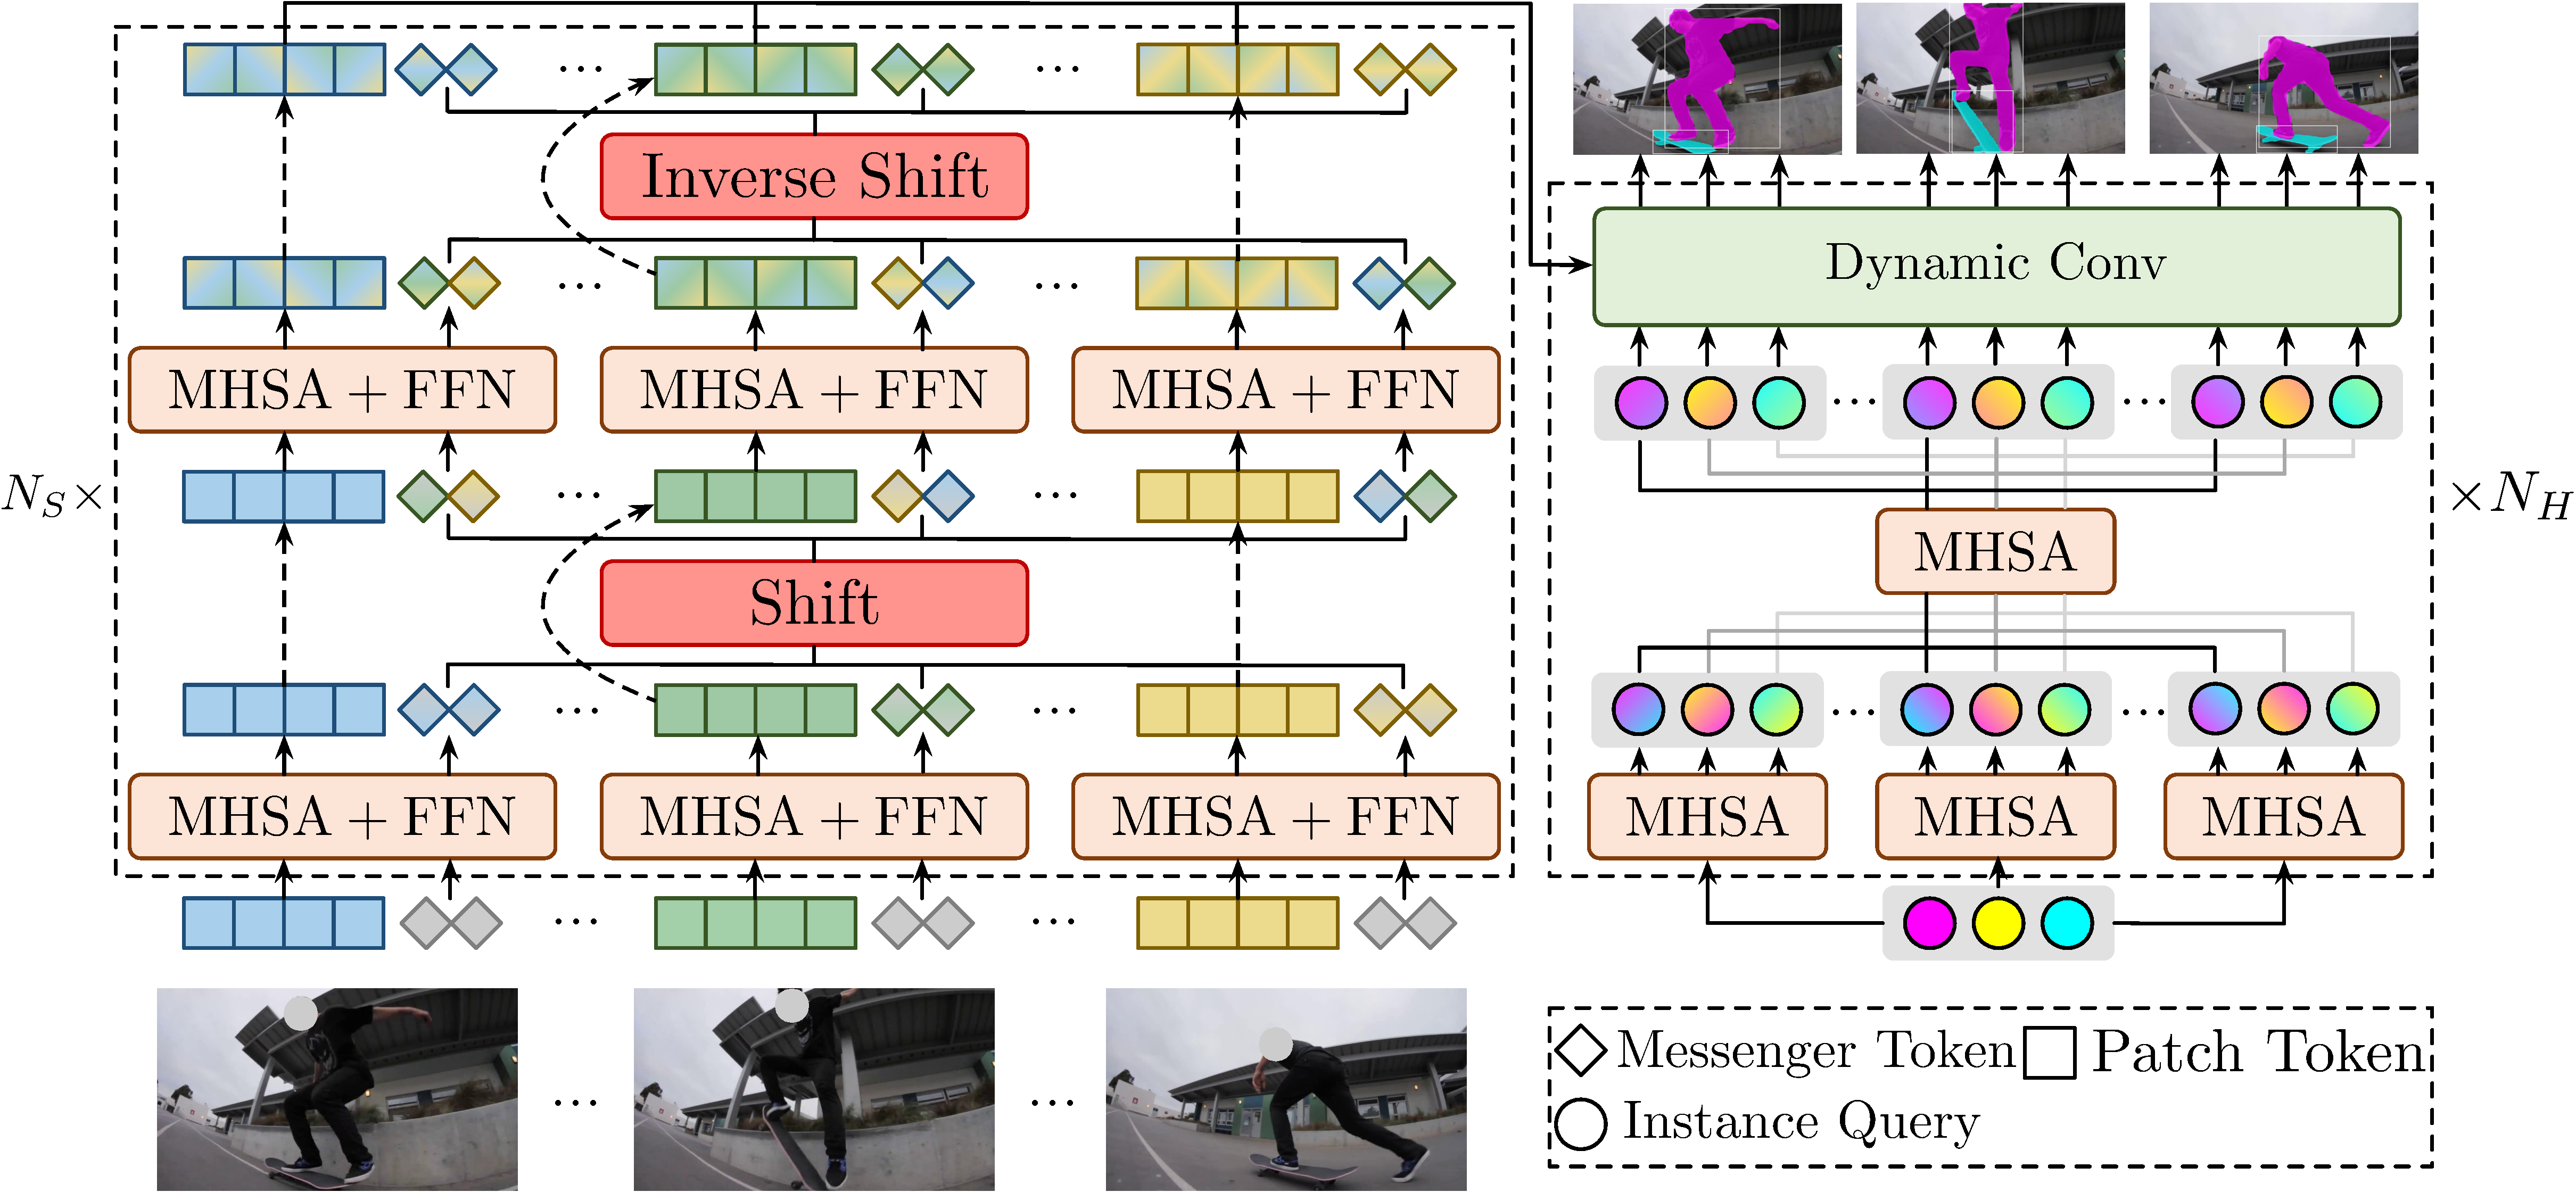
\includegraphics[width=1.0\textwidth]{./images/TeViT_architecture.pdf}
	\caption[Architecture of TeViT]{Architecture of TeViT: The overall illustration of our TeViT framework. TeViT contains a messenger shift transformer backbone and a series of
		spatiotemporal query-driven instance heads. The messenger shift mechanism performs efficient frame-level temporal modeling by simply shifting messenger tokens along the temporal axis. Spatiotemporal query interaction conducts two successive and parameter-shared
		multi-head self-attention (MHSA) with feed forward network (FFN) upon video instance queries. Image and text taken from \cite{yang2022temporallyefficientvisiontransformer}.}
	\label{Architecture_of_TeViT}
\end{figure}





%%%%%%%%%%%%%%%%%%%%%%%%%%%%%%%%%%%%%%%%%%%%%%%%%%%%%%%%%%%%
\subsection{Single-Head Vision-Transformer (SHViT)} \label{sec_architecture_shvit}
Traditional Vision Transformers usually employ $4 \times 4$ patch embeddings, a four-stage backbone architecture, and a multi-head attention mechanism \cite{liu2022convnet2020s, li2022efficientformervisiontransformersmobilenet, vasu2023fastvitfasthybridvision}. In contrast, \gls{shvit} was selected for its memory efficiency in segmentation tasks. In contrast, \gls{shvit} was chosen for its memory efficiency in segmentation tasks, which is partly attributed to its patchify stem that uses larger-stride $16 \times 16$ patch embeddings without sacrificing performance. Additionally, researchers have observed that attention mechanisms in the early stages of the network lead to computational redundancies, which is mitigated by \gls{shvit} by incorporating a single-head attention module \cite{yun2024shvit}.

\medskip 

The \gls{shvit} architecture is composed of a backbone and a decoder. The backbone begins with a $16 \times 16$ overlapping patch embedding block, followed by three \gls{shvit} blocks, each separated by a downsampling layer. The patch embedding is implemented using a sequence of four $3 \times 3$ strided convolutional layers\footnote{It was observed that using a $16 \times 16$ patch embedding block led to an excessive reduction in spatial resolution. Therefore, in this thesis a $4 \times 4$ block (2 convolutional layers instead of 4 convolutional layers) was used instead to preserve more spatial detail. However, the number of layers is parameterizable.}, each configured with a kernel size of $3 \times 3$, a stride of 2, \gls{relu} activation, and Batch Normalization. This setup effectively reduces the spatial dimensions of the input by a factor of 16, resulting in a compact and efficient feature representation as shown in figure \ref{Architecture_of_SHViT}.

\begin{figure}[H]
	\centering
	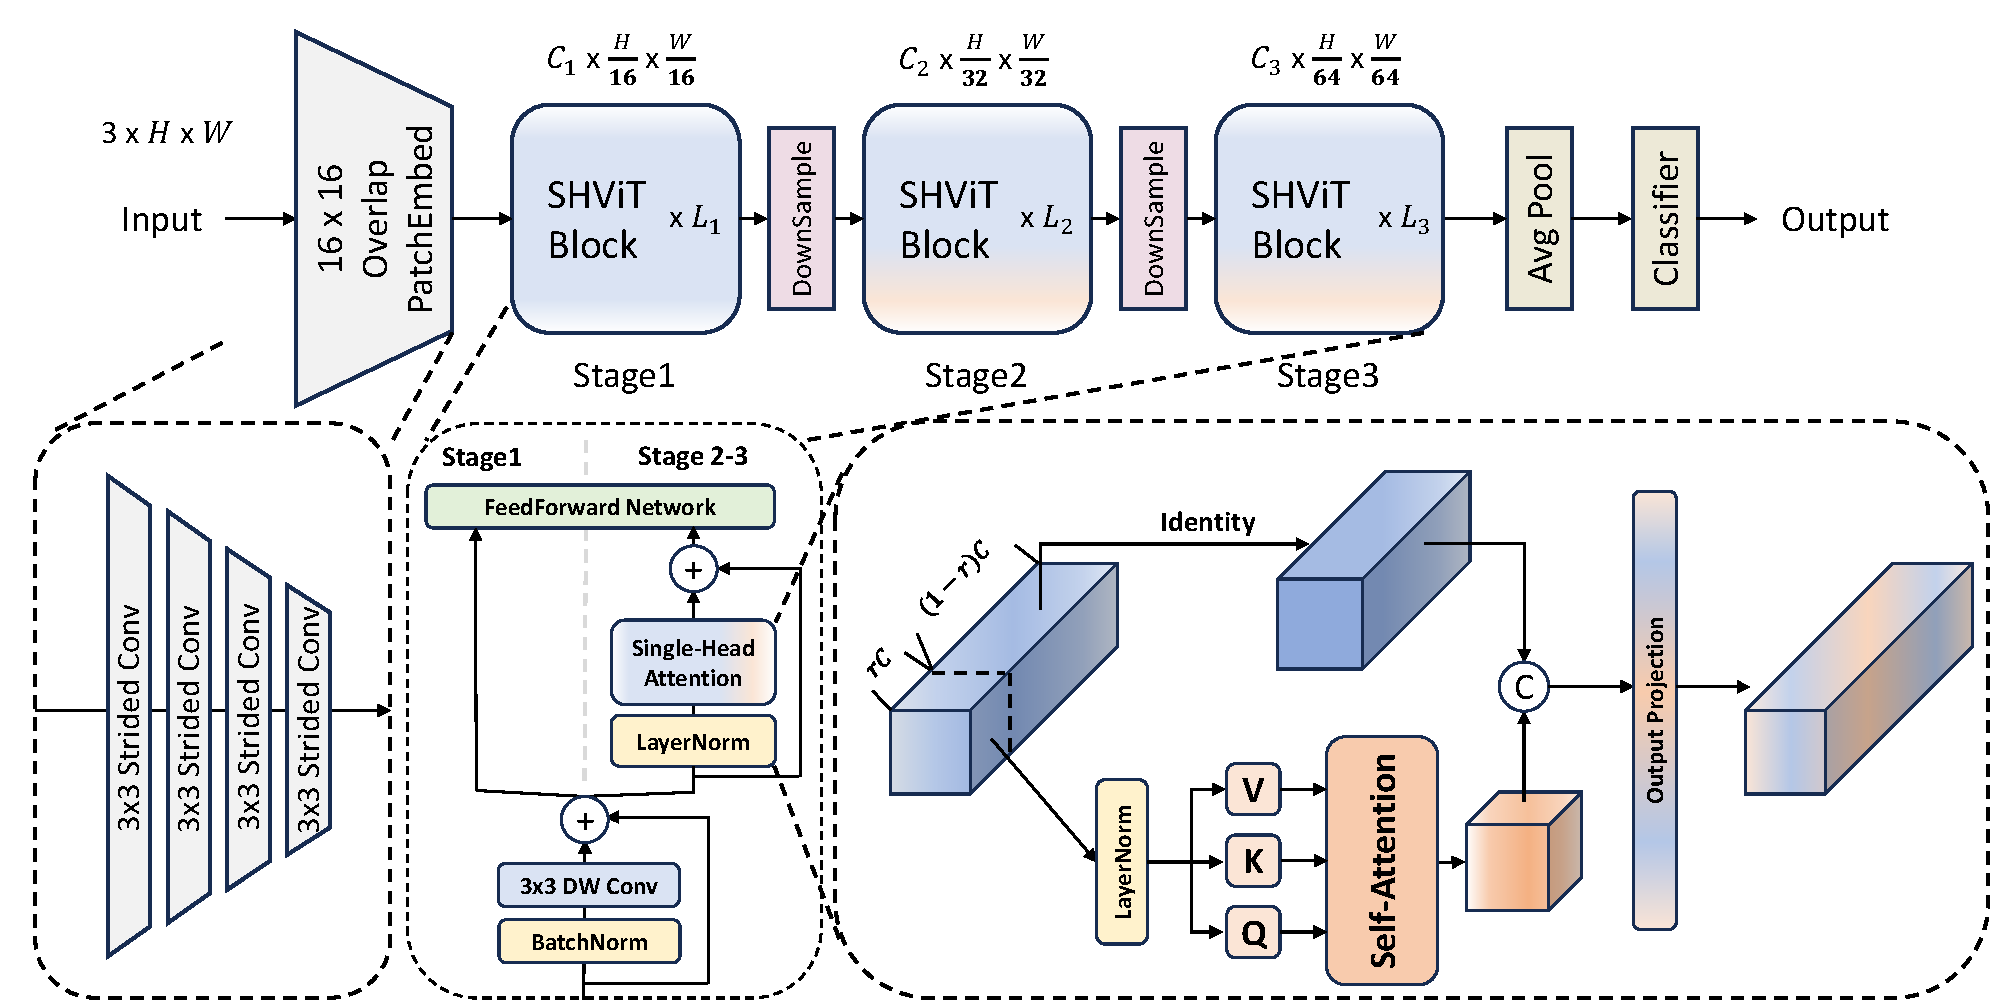
\includegraphics[width=1.0\textwidth]{./images/SHViT_architecture.pdf}
	\caption[Architecture of SHViT]{Architecture of SHViT. Image taken from \cite{yun2024shvit}.}
	\label{Architecture_of_SHViT}
\end{figure}

To optimize computational efficiency, single-head self-attention is intentionally omitted in the early stages of the network and instead introduced in the later stages, where global context modeling is more beneficial. Consequently, the first stage of the \gls{shvit} backbone is designed without attention layers. It comprises Batch Normalization, a $3 \times 3$ depthwise convolution with stride 1 and \gls{relu} activation, and a feedforward network composed of fully connected layers with fused Batch Normalization and \gls{relu} activation. The spatial resolution remains unchanged throughout each individual stage, preserving feature map dimensions for consistent processing.

\medskip

Given that \gls{shvit} is structured with only three stages, the single-head self-attention mechanism is employed exclusively in the second and third stages. It is placed between the depthwise convolution and the feedforward network within each stage. This design enables efficient capture of long-range dependencies and enhances the network's ability to model global context in deeper layers, where such information becomes increasingly relevant. 

\medskip

The output of the backbone is then forwarded to a lightweight decoder, which consists of an average pooling layer followed by a classifier. This final component generates the model's predictions, thereby completing the \gls{shvit} pipeline as illustrated in figure \ref{Architecture_of_SHViT}. It is important to note that the final classification layer of the \gls{shvit} model is omitted, as only the outputs from the three backbone stages are required and subsequently passed to the \gls{mlp} layer of the SegFormer decoder \cite{yun2024shvit} (see also section \ref{sec:segformer}).

\medskip

The version of \gls{shvit} used in this thesis is based on the code from the publicly available GitHub repository\footnote{\url{https://github.com/ysj9909/SHViT/blob/main/model/shvit.py}}, with minor modifications detailed in chapter \ref{code_implementation}, section \ref{sec::shvid_3d.py}. It should be noted that the \enquote{Block} shown in figure \ref{Architecture_of_SHViT} differs from the \enquote{Block} defined in the code. In the code, the \enquote{Block} also includes the downsampling operation, whereas in the diagram, these components are depicted separately.




%%%%%%%%%%%%%%%%%%%%%%%%%%%%%%%%%%%%%%%%%%%%%%%%%%%%%%%%%%%%%%%%%%%%%%%%%%%%%%%%%%%%%%%%%%%%%%%%

\subsection{Choosing the right ViT for 3D volumetric data}
In the previous sections, various \glspl{vit} such as \gls{tevit} \cite{yang2022temporallyefficientvisiontransformer}, \gls{efficientvit} \cite{liu2023efficientvitmemoryefficientvision} \gls{avit} \cite{du2024avitadaptingvisiontransformers}, SegFormer \cite{xie2021segformersimpleefficientdesign}, and \gls{shvit} \cite{yun2024shvit} are described. As noted at the beginning, choosing the right \gls{vit} is critical given the enormous computational and memory demands of processing \gls{3d} data. An equally important criterion is the simplicity and adaptability of the architecture. Unlike \gls{2d} images, volumetric inputs generate a token number that cubically increases with each spatial dimension, rendering standard multi-head self-attention practically useless at comparable resolutions.

\medskip

\gls{avit}, for example, freezes a pre-trained \gls{vit} backbone and uses lightweight prompt embeddings and adapters to adapt to new domains. Nevertheless, \gls{avit} still relies on self-attention across thousands of tokens, resulting in large-scale \gls{gpu} memory requirements even when the volume is scaled down.

\medskip

\gls{efficientvit} employs cascaded group attention, which helps reduce memory access overhead to some extent and saves computation overhead, but still uses an attention mechanism in each stage that leads to computational redundancies that is solved by \gls{shvit} applying a subset of feature channels (partial ratio). Consequently, in practice, batch sizes must be drastically reduced to satisfy hardware constraints, which in turn destabilizes the normalization layers and reduces training throughput.

\medskip

\gls{tevit}'s efficiency advantages are exclusive to two spatial dimensions, making it unsuitable for \gls{3d} voxel data. The \gls{pvt} backbone reduces the number of tokens by patch merging only along the height and width, leaving the depth dimension completely untouched. As a result, the cubic growth of the token length (depth $\times$ height $\times$ width) remains across all \gls{mhsa} layers, which leads to high memory consumption even after downsampling.

\medskip

SegFormer uses four Transformer blocks in its encoder and employs a multi-layer perceptron (\gls{mlp}) layer in the decoder to combine the outputs from each encoder stage and make the final prediction. A major drawback of this design is the large number of trainable parameters, which can reach up to approximately 120 million, significantly increasing the model's computational and memory demands.

\medskip

Unlike other Vision Transformer models, \gls{shvit} does not employ Multi-Head Self-Attention. Instead, it relies on a \gls{shsa} mechanism, which reduces memory consumption and the number of trainable parameters compared to multi-head architectures. By replacing multiple parallel attention heads with a single head, \gls{shvit} not only lowers computational overhead but also limits memory access. In particular, the partial-channel approach illustrated in figure 6 of the original paper \cite{yun2024shvit} directs only a subset of feature channels through the \gls{shsa} modules, while preceding convolutional layers extract local detail. This design achieves \enquote{the best speed-accuracy trade-off}\cite{yun2024shvit} by unifying the complementary strengths of convolution and attention in a single token mixer. At the same time, memory-bound operations such as tensor reshaping and layer normalization are confined to a limited number of channels. As shown in figure 7 of the \gls{shvit}-paper \cite{yun2024shvit}, this allows the \gls{shsa} module to use \gls{gpu} and \acrshort{cpu} compute resources far more efficiently than conventional multi-head mechanisms. By reducing memory-intensive steps, such as reshaping and normalization, the peak memory footprint drops substantially, enabling larger batch sizes and higher image resolutions in volumetric \gls{3d} scenarios while preserving training stability. 



\subsection{Architecture of 3D SHViT-SegFormer} \label{sec:Architecture_of_SHViT_Segformer}
The decoder portion of \gls{shvit} is designed for instance or object detection rather than for semantic segmentation; that's why a different head is required. For this purpose, the head from the SegFormer model \cite{xie2021segformersimpleefficientdesign, perera2024segformer3defficienttransformer3d} was adopted. SegFormer includes both an encoder and a decoder, as do most vision transformers (see figure \ref{Architecture_of_Segformer}). The SegFormer model with \gls{shvit} as its backbone represents a straightforward combination of both individual models. However, since \gls{shvit} consists of only three stages, only three feature maps are forwarded to the \gls{mlp} decoder. The number of convolutional layers $N$ in the Overlap Patch Embedding block is a configurable parameter and can range from 1 to 4. As will be demonstrated in chapter \ref{Results_and_Discussion}, setting {\tt N=2} gives the best trade-off between F1/Dice-performance and \gls{gpu} memory usage.

\medskip

Figure \ref{Architecture_of_SHViT_Segformer} shows the points at which the \gls{shvit} outputs are extracted and transferred to the \gls{mlp} block of the SegFormer decoder.

\begin{figure}[H]
	\centering
	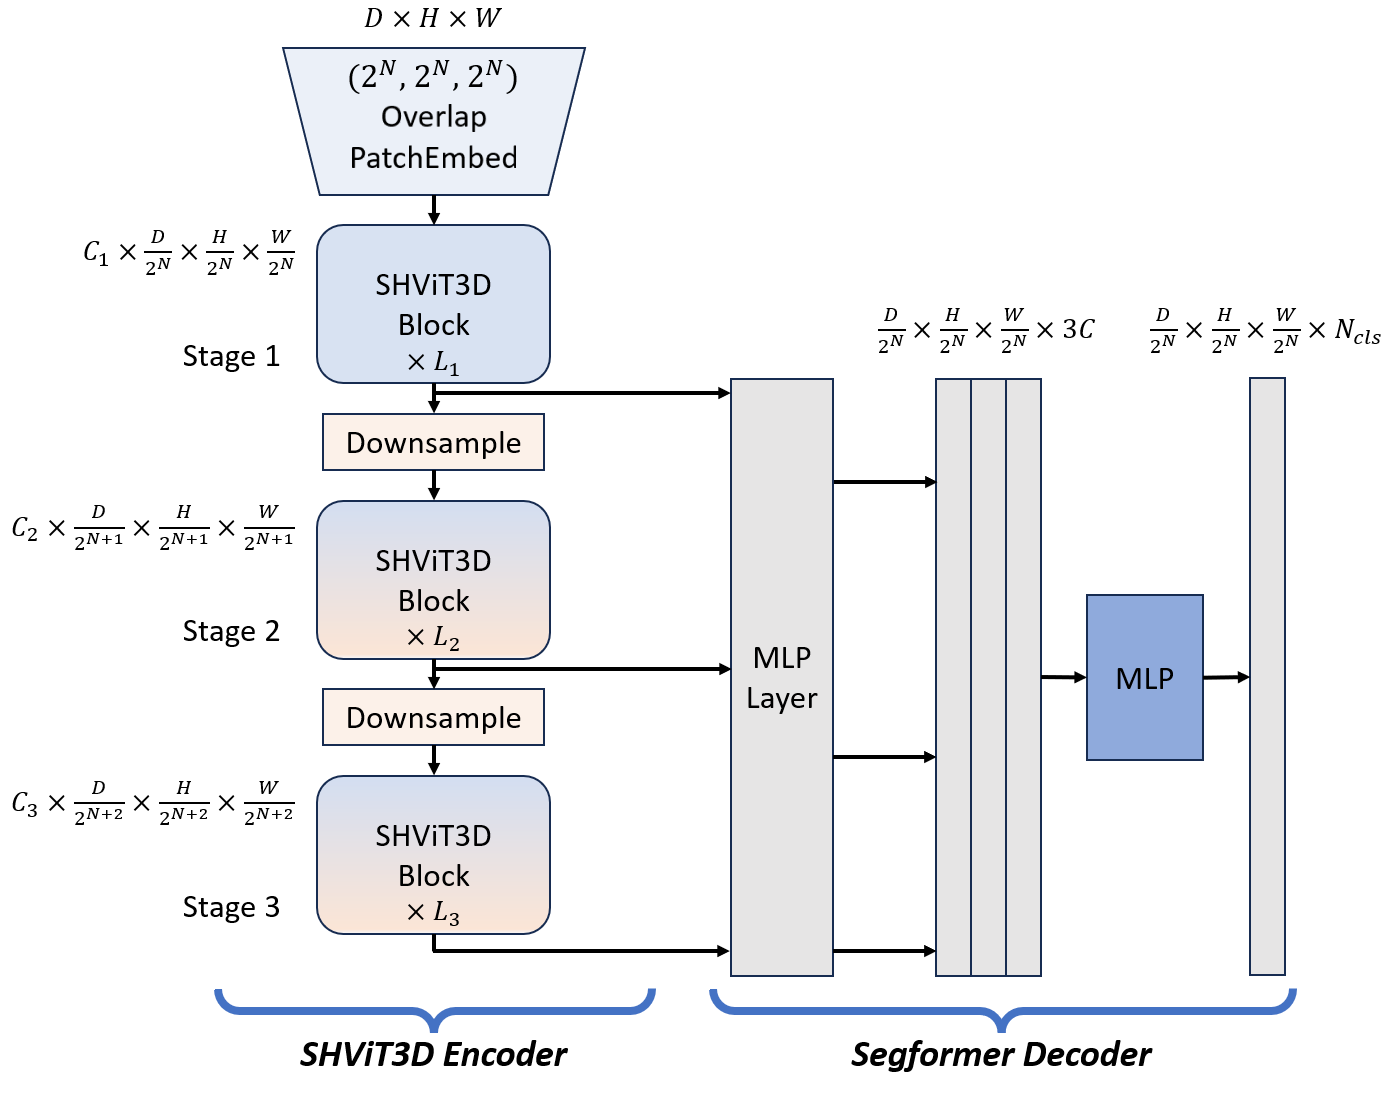
\includegraphics[width=0.9\textwidth]{./images/Architecture_of_SHViT_Segformer.png}
	\caption[Architecture of SegFormer with 3D SHViT-backbone]{Architecture of SegFormer with 3D SHViT-backbone: $N$ is the number of convolutional layers in PatchEmbedding-Block (SHViT3D-head). {\tt stride=2} reduces the size after each downsampling block by a factor of $2$.}
	\label{Architecture_of_SHViT_Segformer}
\end{figure}

According to \cite{xie2021segformersimpleefficientdesign}, Section 4.2 (Ablation Studies: Influence of {\tt C}, the \gls{mlp} decoder channel dimension), the SegFormer decoder uses an {\tt embed\_dim} of {\tt 256} for variants B0 and B1, and {\tt 768} for B2 through B5. The parameter settings for the \gls{3d} \gls{shvit} component of the model are presented in table \ref{tab:variants}, which is adapted from \cite{yun2024shvit, IMvision12}.

\begin{center}
	\begin{threeparttable}[H]
	\begin{tabular}{l|cc|c|c|c|c}
		\toprule
		\multicolumn{1}{c|}{Model variants} & Depth     & Emb.~dim.       & Partial ratio              & Exp.~ratio         & B0/B1                & B2-B5                \\
		\midrule
		\midrule
		SHViT-S1                            & [2, 4, 5] & [128, 224, 320] &  \multirow{4}{*}{1 / 4.67} & \multirow{4}{*}{2} & \multirow{4}{*}{256} & \multirow{4}{*}{768} \\
		SHViT-S2                            & [2, 4, 5] & [128, 308, 448] &                            &                    &                      &                      \\
		SHViT-S3                            & [3, 5, 5] & [192, 352, 448] &                            &                    &                      &                      \\
		SHViT-S4                            & [4, 7, 6] & [224, 336, 448] &                            &                    &                      &                      \\ 
		\bottomrule
	\end{tabular}
	\caption[Architecture details of 3D SHViT variants]{Architecture details of 3D SHViT variants: table taken from \cite{yun2024shvit}. Parameters B0 to B5 are used in {\tt embed\_dim} of SegFormer decoder, values are taken from \cite{IMvision12}.}
	\label{tab:variants}	
	\end{threeparttable}
\end{center}



\section[Reducing Memory in Transformer Attention Mechanisms]{Reducing Memory in Transformer Attention \\ Mechanisms} \label{Transformer_Attention_Mechanisms}
The self-attention mechanism\footnote{In the original Transformer paper by Vaswani et al. \cite{vaswani2023attentionneed}, the attention score is written as $qk^T$, since the query and key matrices are typically shaped $(n,d_k)$, placing the sequence length $n$ first. However, in the codebase for \gls{shvit}, the tensor shape is just opposite: $(d_k,n)$. This reverses the usual convention, and to be consistent with the code, $q^Tk$ is used in this thesis.}, particularly the computation of 
\begin{equation}
	\text{Attention}(q, k, v) = \text{softmax}\left(\frac{q^T k}{\sqrt{d_k}}\right)v
\end{equation}
can be highly memory-intensive, especially when processing long sequences or high-dimensional embeddings \cite{vaswani2023attentionneed}. The high memory consumption comes from the matrix multiplication between the transposed query tensor ({\tt q}) and the key tensor ({\tt k}), which is of order $O(n^2)$. The term $d_k$, representing the dimensionality of the queries and keys, will later be denoted as {\tt qk\_dim}. To understand the impact, it is important to consider the shapes and scaling behavior of these tensors. The following explanation, based on the \gls{shvit} architecture with the S4 configuration, illustrates the reasons behind the large sizes of the query, key, and value matrices denoted as {\tt q}, {\tt k}, and {\tt v}. In the following, the operations that take place within the \gls{shsa} block are described. The corresponding code implementation can be found in section \ref{sec::shvid_3d.py} in the {\tt SHSA3D} class.


\subsection{Memory Bottleneck in 3D Attention Block}
Starting with an input volume of shape {\tt (1,224,224,224)}, where the first dimension indicates the batch size,  and using for the calculation two {\tt Conv3D} layers in the {\tt PatchEmbed} head (see figure \ref{Architecture_of_SHViT_Segformer}), the spatial dimensions are downsampled by a factor of 2 at each layer, resulting in an intermediate feature map of shape {\tt (1,56,56,56)}. This tensor is then passed into the first {\tt SHViT3D} block, where another spatial downsampling by a factor of 2 is performed, reducing the shape to {\tt (1,28,28,28)}. At this point, the channel dimension is expanded to {\tt 336}, creating a tensor of shape {\tt (1,336,28,28,28)} as the input to the forward function of the {\tt SHSA3D} module.

\medskip

Within the forward function, the input tensor {\tt x} has the shape {\tt (1,336,28,28,28)}. The following S4-configuration parameters are used:
\begin{itemize}
	\item {\tt dim = 336} (input channels),
	\item {\tt qk\_dim = 16} (dimension of queries and keys),
	\item {\tt pdim = 72}, which corresponds to a fraction of approximately ${1}/{4.7}$ of the total channels of {336}.
\end{itemize}

\noindent The tensor {\tt x} is then split along the channel dimension into two parts:
\begin{itemize}
	\item {\tt x1} with shape {\tt (1,72,28,28,28)} (used for computing attention),
	\item {\tt x2} with shape {\tt (1,264,28,28,28)} (bypasses attention and is later concatenated back).
\end{itemize}
Next, the tensor {\tt x1} is passed through the {\tt qkv} layer, which is essentially a {\tt Conv3D} with input channels of {\tt 72} and output channels of {\tt 2*qk\_dim + pdim = 2*16 + 72 = 104}. This produces a tensor of shape {\tt (1,104,28,28,28)}, which is then split into
\begin{itemize}
	\item query tensor {\tt q} with shape {\tt (1,16,28,28,28)},
	\item key tensor {\tt k} with shape {\tt (1,16,28,28,28)},
	\item value tensor {\tt v} with shape {\tt (1,72,28,28,28)}.
\end{itemize}
After flattening the spatial dimensions, the shapes become
\begin{itemize}
	\item {\tt q} with shape {\tt (1,16,21952)},
	\item {\tt k} with shape {\tt (1,16,21952)},
	\item {\tt v} with shape {\tt (1,72,21952)}.
\end{itemize}
where {\tt 21952} is simply $28^3$, the total number of voxels of this stage.

\medskip

The critical and memory-intensive operation that follows now performs matrix multiplication between tensors {\tt q$^{\text{\tt T}}$} and {\tt k} of shapes {\tt (1,21952,16)} and {\tt (1,16,21952)}, respectively, producing an attention matrix of shape {\tt (1,21952,21952)}, containing over 480 million elements. This quadratic growth in memory usage, relative to the spatial size, is the primary source of computational bottleneck in the model.

\medskip

Subsequently, the final attention-weighted values are computed by multiplying the value tensor {\tt v} to the matrix, which reduces the tensor back to shape {\tt (1,72,21952)}, and after reshaping, results in its final size of {\tt (1,72,28,28,28)}. Finally, this attention-modified output is concatenated along the channel dimension with the unmodified {\tt x2}, reconstructing the full tensor with shape {\tt (1,336,28,28,28)} for further processing (see also figure \ref{Architecture_of_SHViT}). This detailed tracing highlights not only the shape transformations but also the source of the heavy memory usage, the large attention matrix, which becomes especially problematic for high-resolution \gls{3d} volumes.

\medskip

However, if only one single {\tt Conv3D} layer is used in the head of the {\tt SHViT3D} model, resulting in a reduced downsampling, or if the input volume size is doubled, then the input to the {\tt SHSA3D} block increases in spatial resolution. In this case, the input shape becomes {\tt (1,336,56,56,56)}, and the resulting attention matrix grows to a size of {\tt ({56$^3$},{56$^3$}) = (175616,175616)}, which contains over 30 billion elements. This represents a 64 increase in memory consumption compared to the previous case, highlighting the exponential scaling behavior of the attention mechanism in \gls{3d} space.

\medskip

This observation clearly illustrates why the {\tt SHViT3D} model, particularly the {\tt SHSA3D} block, is highly memory-intensive. Careful architectural decisions are necessary to balance segmentation quality and memory feasibility. In practice, using two {\tt Conv3D} stages in the head provides a good compromise, sufficient downsampling to reduce memory usage while still preserving enough spatial detail for accurate segmentation.

\bigskip

Several strategies have been proposed in the literature to reduce memory consumption while preserving model performance. The following techniques are commonly used:

\begin{itemize}
	\item Precision Reduction: Use lower precision data types, like {\tt float8} or {\tt float16} instead of {\tt float32}, to reduce the memory consumption with minimal accuracy loss \cite{Bravin_2025}. A further reduction in quantization down to 4- or 2-bit was also studied in \cite{Shen_2020}. The implementation of mixed-precision computation has proven to be an effective strategy for reducing memory consumption during model training and inference. In this thesis, mixed-precision training was adapted to optimize the memory efficiency of the model within the available hardware constraints. The code uses the {\tt Lightning} library from {\tt Fabric} to facilitate and manage mixed-precision training efficiently\footnote{\url{https://lightning.ai/docs/fabric/stable/fundamentals/precision.html}}.

	\item Perform Attention on Smaller Blocks: Divide the input sequences into smaller blocks and perform attention on these blocks separately. This approach, known as \enquote{block sparse attention}, \enquote{local attention}, or \enquote{sliding-window}, reduces matrix size. For example, Longformer replaces full attention with a sliding-window local attention plus a few global tokens. This makes memory scale linearly with sequence length \cite{beltagy2020longformerlongdocumenttransformer}. This idea was implemented using the code snippet from \acrshort{simvit} \cite{Li_2022} and is described further below.
	
	\item Use of Sparse Matrices: If the matrices contain many zeros or negligible values, using sparse matrix representations could save memory. Literature research shows that Child et al.~\cite{Child_2019} introduced Sparse Transformers that attend with fixed strided and block-sparse patterns. Sparse matrices typically maintain accuracy comparable to dense attention and in some cases even improve training speed, at the cost of introducing heuristic patterns or additional overhead from sorting or clustering \cite{Deepspeed_2020}. Due to its high complexity, it was not implemented in the code.
\end{itemize}



\subsection{Sliding-Windows Mechnism}
Due to the fact that spatially distant regions in an image generally do not exhibit strong relationships, it is reasonable to process images using a sliding window approach with overlapping regions. This method enables the efficient capture of local spatial structures by focusing only on a patch and its immediate neighbors while ignoring distant points (or tokens) \cite{fu2025slidingwindowattentiontraining}. Within each window, as shown in figure \ref{Sliding_Window}, a \gls{shcsa} mechanism is applied, where only the central patch serves as the query, and the surrounding patches are used as keys and values. While the original method is based on \gls{mhcsa} as suggested by Li et al.~in the \acrshort{simvit} paper \cite{Li_2022}, this thesis modifies the idea by taking just the attention part from \gls{mhcsa} and combining it with \gls{shsa} from \gls{shvit}. This results in an enhanced version, referred to as \gls{shcsa}, which significantly reduces computational cost while maintaining a high level of performance and accuracy.

\begin{figure}[H]
	\centering
	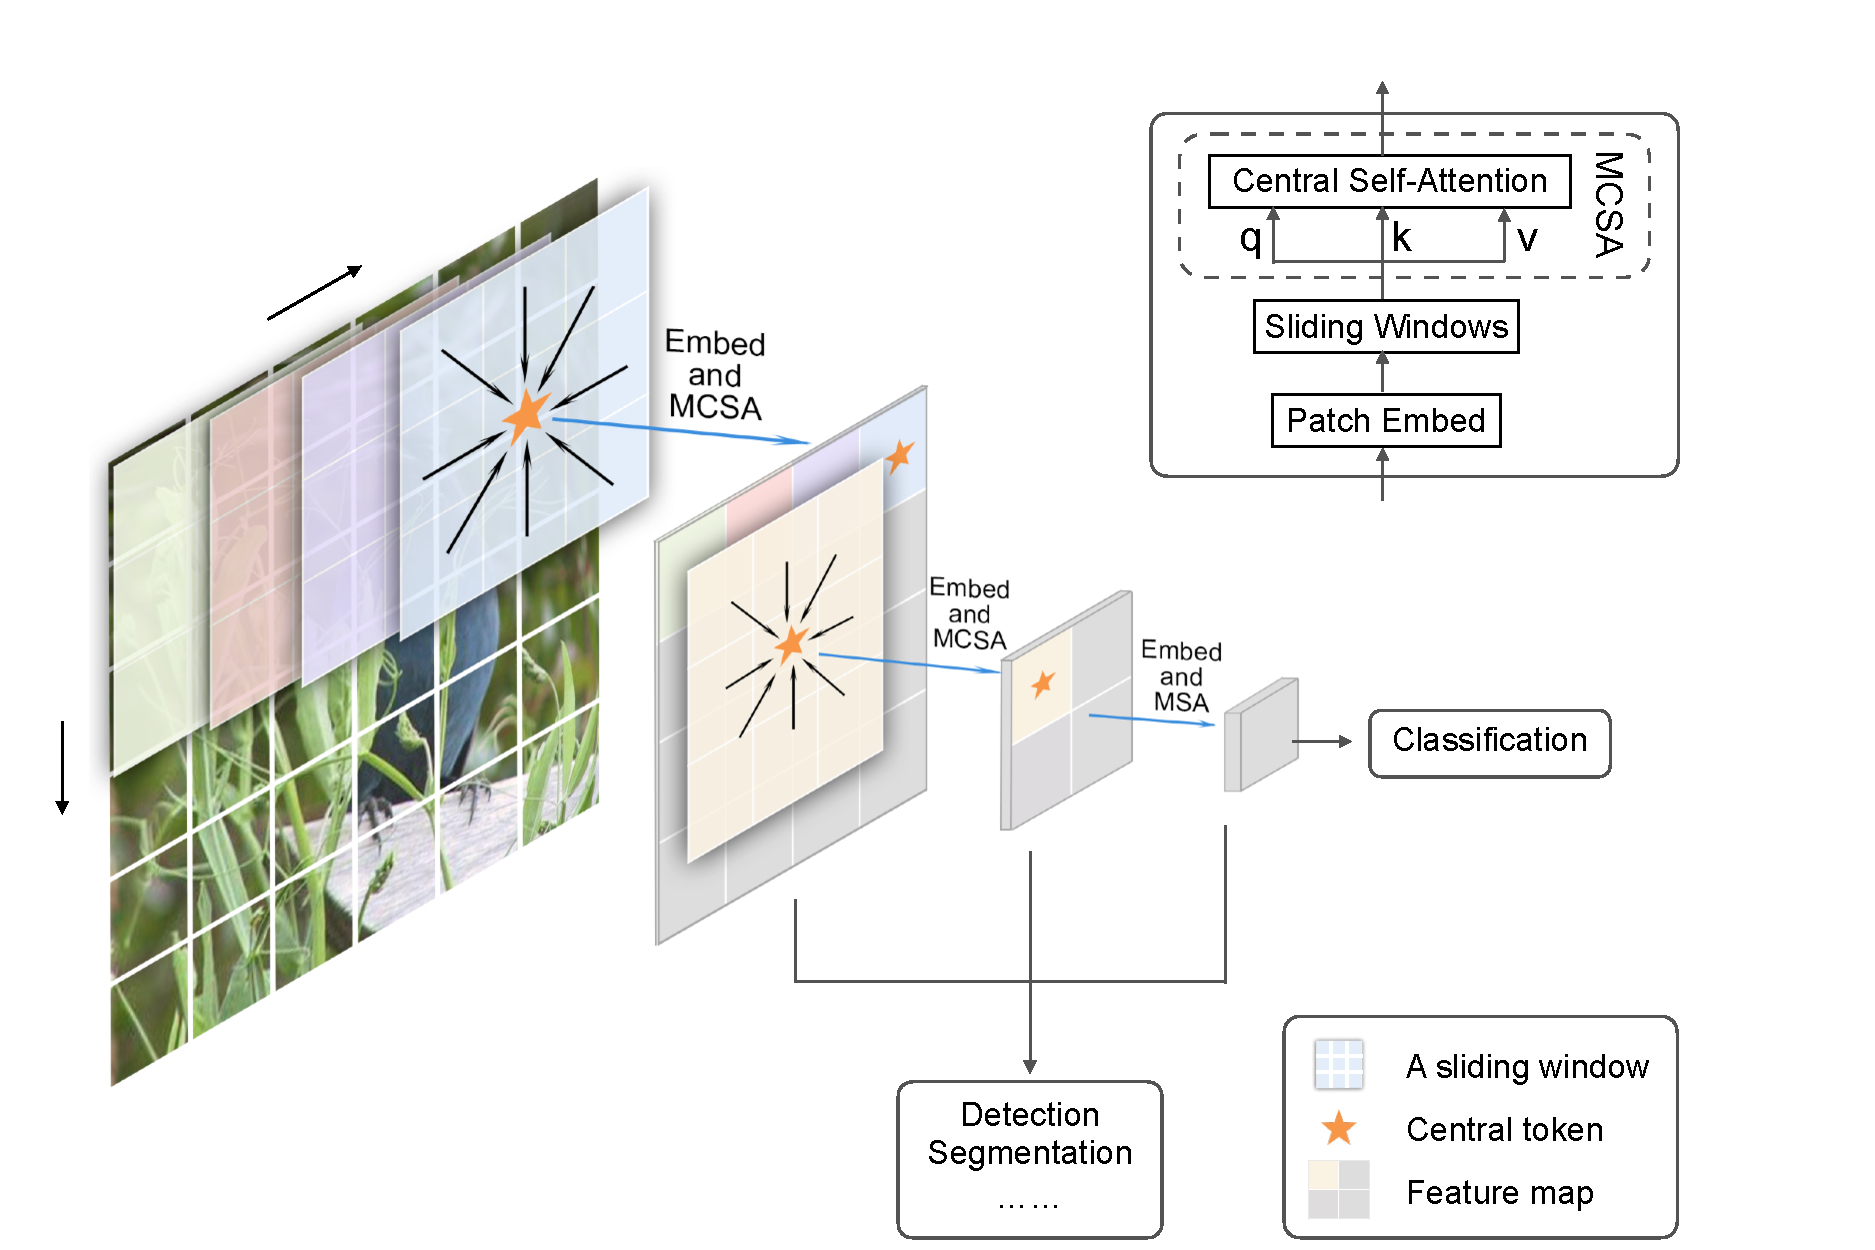
\includegraphics[width=0.9\textwidth]{./images/motivation6.pdf}
	\caption[Visualisation of the sliding window mechanism]{Visualisation of the sliding window mechanism with overlapping regions applied to the feature map of the image. Within each window, only the central patch (highlighted) acts as the query, while the neighboring patches serve as keys and values. Image taken from \cite{fu2025slidingwindowattentiontraining}.}
	\label{Sliding_Window}
\end{figure}



\section{Metrics Used for Model Evaluation}
In the context of neural network training, metrics and loss functions play an important role in guiding the optimization process and evaluating model performance. 

\medskip

\noindent Evaluating the performance of segmentation models involves several metrics, including \cite{azad2023lossfunctionserasemantic}:

\medskip

{\bf \gls{iou}} or {\bf Jaccard index}, which is the ratio of the intersection area to the union area of the predicted ($P$) and ground truth segments ($G$): 
\begin{equation}
	\text{IoU} = \frac{\left| P \cap G \right|}{\left| P \cup G \right|} = \frac{\left| P \cap G \right|}{\left| P \right| + \left| G \right| - \left| P \cap G \right|}
\end{equation}
The Jaccard Distance Loss is the defined as
\begin{equation}
	\text{Jaccard-Distance-Loss} = 1 - \text{IoU}
\end{equation} 
If there is no intersection between the two classes $P$ and $G$, then $\left| P \cap G \right| = 0$ and $\text{IoU}=0$ and the $\text{Jaccard-Distance-Loss} = 1$. In an experiment with multiple segmentations, \gls{iou} is averaged over all single \glspl{iou}: 
\begin{equation}
	\text{mIoU} = \frac{1}{N} \sum_{i=1}^N \text{IoU}_i
\end{equation}

\medskip

An often used overlap metric is the {\bf Dice Coefficient}. It is defined by the following formula (where $P$ are the predicted and $G$ are the ground truth segments):
\begin{align}
	\text{Dice} &= \frac{2 \left| P \cap G \right|}{\left| P \right| + \left| G \right|} \\
	&= \frac{2 \cdot \text{IoU}}{1 + \text{IoU}}
\end{align}
and the Dice-Loss is then defined as 
\begin{equation}
	\text{Dice-Loss} = 1 - \text{Dice}
\end{equation} 

The Dice coefficient is closely related to the F1-score used in classification tasks. In the binary case, they are mathematically equivalent when precision and recall are defined as $\text{precision} = {|P \cap G|}/{|P|}$ and $\text{recall} = {|P \cap G|}/{|G|}$, respectively. However, they are applied in different contexts: Dice is used in segmentation, where predictions are made at the pixel or voxel level, whereas the F1-score is used in classification settings, such as token-level or object-level evaluation \cite{taha2015metrics, saito2015precision}. In multi-class scenarios or with weighted averaging, differences in implementation may arise.

\medskip

Dice/F1 and \gls{iou} are monotonically related, so a better overlap raises both scores. However, Dice/F1 tends to be higher for the same overlap (e.g.~$\text{IoU}=0.5 \rightarrow \text{Dice/F1} \approx 0.67$). This means that Dice/F1 places greater emphasis on the intersection, whereas \gls{iou} penalizes false positives and false negatives more heavily, similar to how L2 loss emphasizes large deviations compared to L1. In non-medical computer vision, \gls{iou} or \acrshort{miou} is predominantly used as the evaluation metric, particularly in object detection, while Dice-based loss functions are mostly used during training for segmentation tasks, particularly when there are imbalances in class sizes or when objects are small \cite{azad2023lossfunctionserasemantic}. 

\medskip

Additionally, both metrics can be misleading when averaged across many samples, especially when ground truth regions are tiny. In such cases, even minor errors can disproportionately reduce the overall score, giving excessive weight to trivial misclassifications.

\medskip

Another loss function, which can be used for image segmentation, is the {\bf cross-entropy} loss. It also measures the difference between predictions and ground truth but treats each pixel independently, regardless of the class it belongs to. Therefore, it is very sensitive to class imbalance unless it is weighted. For example, in imbalanced datasets with a lot of background in the image/volume, the cross-entropy loss is very much influenced by the majority class. As a result, the model may learn to prioritize accuracy on the frequent classes while ignoring others. In contrast, Dice/F1 and \gls{iou} losses measure the overlap between predicted and true regions and therefore offer better performance on imbalanced datasets \cite{azad2023lossfunctionserasemantic}.

\bigskip

While the F1-score and Dice coefficient are mathematically equivalent for binary segmentation tasks, they differ in origin and usage. F1-score comes from information retrieval and is widely used in machine learning, while the Dice coefficient originated in ecological studies \cite{enwiki:1297073156} and is commonly used in medical image segmentation \cite{taha2015metrics}. In multi-class settings, the F1-score typically uses standardized averaging methods (e.g., macro or micro), whereas Dice averaging can vary across implementations \cite{yeung2021unified}. The F1-score is also more broadly recognized in general machine learning, while Dice remains standard in medical imaging \cite{Reinke_2024}. This thesis uses the F1-score for its wider recognition and consistent definition.
